\documentclass{beamer}
\usepackage{soton-beamer}
\usepackage{winfonts}
\renewcommand{\sfdefault}{georgia}

\title{Identification of the Curie Temperature Distribution from
Temperature Dependent Magnetisation Data}
\author{Jonathon Waters\inst{1}, Hans Fangohr\inst{1}, Denis Kramer\inst{1}\\and Ondrej Hovorka\inst{1}}
\institute{
	\inst{1}
	Engineering and the Environment,\\
	University of Southampton,\\
	UK
}

\begin{document}
\frame{\titlepage 
\includegraphics[width=4cm]{Images/uos_grey_large}}

\setbeamertemplate{headline}{
	\vskip25pt % horizontal line
	\vskip-21pt\hspace{2pt}\hfill
\includegraphics[width=4cm]{Images/uos_grey_large}\hspace{3.5mm} % logo on the right
}

\setbeamertemplate{footline}{
	\vskip-8pt % horizontal line
	\hspace{7.5mm}
	\insertshorttitle
	\hspace{1cm} \insertframenumber/\inserttotalframenumber
	\vskip4pt
}

\begin{frame}
	\frametitle{Introduction}
	\begin{columns}
		\column{7cm}
		\begin{itemize}
		\item{HAMR material can be thought of as a collection of disconnected grains, each with different size $D$.}
		\item{This distribution in $D$ leads to a distribution in the Curie Temperatures $T_C$ of the grains.}
		\item{The distribution in $T_C$ increases the DC noise for the material.}
		\item{According to a 2014 publication, understanding the distribution $f(T_C)$ is a key step to realising HAMR.}
		\end{itemize}
		\column{5cm}
		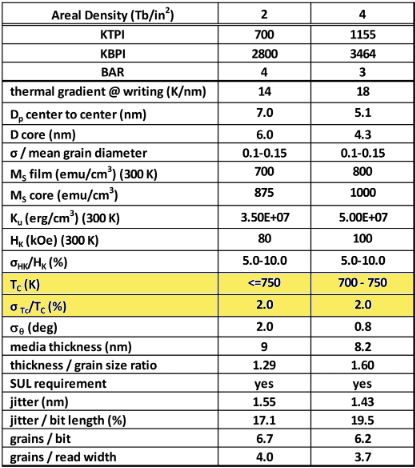
\includegraphics[width=5cm]{Images/Table}
	\end{columns}
\end{frame}

\begin{frame}
	\frametitle{Previous Methods}
\end{frame}

\begin{frame}
	\frametitle{Objectives}
\end{frame}

\begin{frame}
	\frametitle{Our Method}
\end{frame}

\begin{frame}
	\frametitle{Test Case: Ising Model}
\end{frame}

\begin{frame}
	\frametitle{Results}
\end{frame}

\begin{frame}
	\frametitle{Conclusions}
\end{frame}

\begin{frame}
	\frametitle{Acknowledgements}
	In the completion of this work, we acknowledge financial support from the EPSRC Centre for Doctoral Training grant EP/L006766/1. \newline
	
	We also acknowledge the use of the IRIDIS High Performance Computing Facility, and associated support services at the University of
Southampton. \newline

	Contact: J.M.Waters@soton.ac.uk
\end{frame}
\end{document}